% Author: Izaak Neutelings (September 2020)
\documentclass[border=3pt,tikz]{standalone}
\usepackage{physics}
\usepackage{tikz}
\usepackage[outline]{contour} % glow around text
\usetikzlibrary{patterns,snakes}
\usetikzlibrary{arrows.meta} % for arrow size
\contourlength{0.4pt}

\colorlet{xcol}{blue!70!black}
\colorlet{darkblue}{blue!40!black}
\colorlet{myred}{red!65!black}
\tikzstyle{mydashed}=[xcol,line width=0.25,dash pattern=on 2.2pt off 2.2pt]
\tikzstyle{axis}=[->,thick] %line width=0.6
\tikzstyle{ell}=[{Latex[length=3.3,width=2.2]}-{Latex[length=3.3,width=2.2]},line width=0.3]
\tikzstyle{dx}=[-{Latex[length=3.3,width=2.2]},darkblue,line width=0.3]
\tikzstyle{ground}=[preaction={fill,top color=black!10,bottom color=black!5,shading angle=20},
                    fill,pattern=north east lines,draw=none,minimum width=0.3,minimum height=0.6]
\tikzstyle{mass}=[line width=0.6,red!30!black,fill=red!40!black!10,rounded corners=1,
                  top color=red!40!black!20,bottom color=red!40!black!10,shading angle=20]
\tikzstyle{spring}=[line width=0.8,blue!7!black!80,snake=coil,segment amplitude=5,segment length=5,line cap=round]
\tikzset{>=latex} % for LaTeX arrow head
\tikzstyle{force}=[->,myred,very thick,line cap=round]
\def\tick#1#2{\draw[thick] (#1)++(#2:0.1) --++ (#2-180:0.2)}

\begin{document}


% HORIZONTAL spring
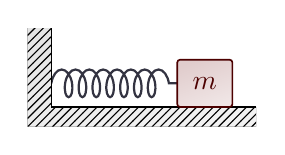
\begin{tikzpicture}
  \def\H{1}    % wall height
  \def\T{0.3}  % wall thickness
  \def\W{2.6}  % ground length
  \def\D{0.25} % ground depth
  \def\h{0.6}  % mass height
  \def\w{0.7}  % mass width
  \def\x{1.6}  % mass x position
  \draw[spring] (0,\h/2) --++ (\x,0);
  \draw[ground] (0,0) |-++ (-\T,\H) |-++ (\T+\W,-\H-\D) -- (\W,0) -- cycle;
  \draw (0,\H) -- (0,0) -- (\W,0);
  \draw[mass] (\x,0) rectangle++ (\w,\h) node[midway] {$m$};
\end{tikzpicture}


% HORIZONTAL spring - axis, rest position
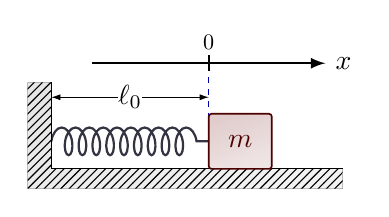
\begin{tikzpicture}
  \def\H{1.1}  % wall height
  \def\T{0.3}  % wall thickness
  \def\W{3.7}  % ground length
  \def\D{0.25} % ground depth
  \def\h{0.7}  % mass height
  \def\w{0.8}  % mass width
  \def\x{2.0}  % mass x position
  \def\y{1.22*\H} % x axis y position
  
  % AXIS
  \draw[mydashed] (\x,0.9*\h) --++ (0,\y-0.9*\h);
  \draw[axis] (\x-0.4*\W,\y) -- (\x+0.4*\W,\y) node[right] {$x$};
  \tick{\x,\y}{-90} node[scale=0.8,above=-1] {$0$};
  \draw[ell] (0,1.3*\h) --++ (\x,0) node[midway,fill=white,inner sep=0] {$\ell_0$};
  
  % SPRING & MASS
  \draw[spring] (0,\h/2) --++ (\x,0);
  \draw[ground] (0,0) |-++ (-\T,\H) |-++ (\T+\W,-\H-\D) -- (\W,0) -- cycle;
  \draw (0,\H) -- (0,0) -- (\W,0);
  \draw[mass] (\x,0) rectangle++ (\w,\h) node[midway] {$m$};
  
\end{tikzpicture}


% HORIZONTAL spring - axis, extended
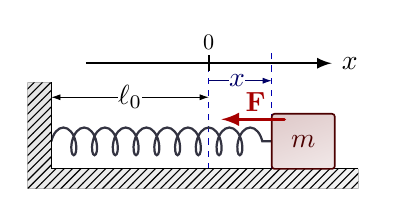
\begin{tikzpicture}
  \def\H{1.1}  % wall height
  \def\T{0.3}  % wall thickness
  \def\W{3.9}  % ground length
  \def\D{0.25} % ground depth
  \def\h{0.7}  % mass height
  \def\w{0.8}  % mass width
  \def\x{2.0}  % mass x position
  \def\dx{0.8} % extension
  \def\y{1.22*\H} % x axis y position
  \def\F{0.8}  % force
  
  % AXIS
  \draw[mydashed] (\x,0) --++ (0,\y) (\x+\dx,0) --++ (0,1.1*\y);
  \draw[axis] (\x-0.4*\W,\y) -- (\x+0.4*\W,\y) node[right] {$x$};
  \tick{\x,\y}{-90} node[scale=0.8,above=-1] {$0$};
  \draw[ell] (0,1.3*\h) --++ (\x,0) node[midway,fill=white,inner sep=0] {$\ell_0$};
  \draw[dx] (\x,1.6*\h) --++ (\dx,0) node[pos=0.45,fill=white,inner sep=0] {$x$};
  
  % SPRING & MASS
  \draw[spring,segment length=7.5] (0,\h/2) --++ (\x+\dx,0);
  \draw[ground] (0,0) |-++ (-\T,\H) |-++ (\T+\W,-\H-\D) -- (\W,0) -- cycle;
  \draw (0,\H) -- (0,0) -- (\W,0);
  \draw[mass] (\x+\dx,0) rectangle++ (\w,\h) node[midway] {$m$};
  \draw[force] (\x+\dx+0.2*\w,0.9*\h) --++ (-\F,0) node[midway,right=1,above=-1] {$\vb{F}$};
  
\end{tikzpicture}


% HORIZONTAL spring - axis, compressed
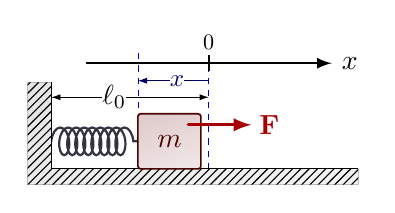
\begin{tikzpicture}
  \def\H{1.1} % wall height
  \def\T{0.3} % wall thickness
  \def\W{3.9} % ground length
  \def\D{0.2} % ground depth
  \def\h{0.7} % mass height
  \def\w{0.8} % mass width
  \def\x{2.0} % mass x position
  \def\dx{0.9} % extension
  \def\y{1.22*\H} % x axis y position
  \def\F{0.8} % force
  
  % AXIS
  \draw[mydashed] (\x,0) --++ (0,\y) (\x-\dx,0) --++ (0,1.1*\y);
  \draw[axis] (\x-0.4*\W,\y) -- (\x+0.4*\W,\y) node[right] {$x$};
  \tick{\x,\y}{-90} node[scale=0.8,above=-1] {$0$};
  \draw[ell] (0,1.3*\h) --++ (\x,0) node[pos=0.4,fill=white,inner sep=0] {$\ell_0$};
  \draw[dx] (\x,1.6*\h) --++ (-\dx,0)
    node[pos=0.45,fill=white,inner sep=0,scale=0.9] {$x$};
  
  % SPRING & MASS
  \draw[spring,segment length=2.9] (0,\h/2) --++ (\x-\dx,0);
  \draw[ground] (0,0) |-++ (-\T,\H) |-++ (\T+\W,-\H-\D) -- (\W,0) -- cycle;
  \draw (0,\H) -- (0,0) -- (\W,0);
  \draw[mass] (\x-\dx,0) rectangle++ (\w,\h) node[midway] {$m$};
  \draw[force] (\x-\dx+0.8*\w,0.8*\h) --++ (\F,0) node[below=0,right=-1] {$\vb{F}$};
  
\end{tikzpicture}


% VERTICAL spring
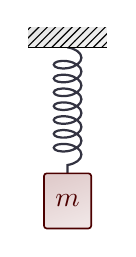
\begin{tikzpicture}
  \def\H{0.25} % ceiling height
  \def\W{1.0}  % ceiling width
  \def\h{0.7}  % mass height
  \def\w{0.6}  % mass width
  \def\y{1.6}  % mass width
  \draw[spring] (0,0) -- (0,-\y);
  \draw[ground] (-\W/2,0) rectangle++ (\W,\H);
  \draw (-\W/2,0) --++ (\W,0);
  \draw[mass] (-\w/2,-\y) rectangle++ (\w,-\h) node[midway] {$m$};
\end{tikzpicture}


% VERTICAL spring - no mass
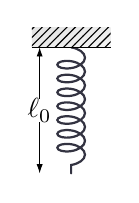
\begin{tikzpicture}
  \def\H{0.25} % ceiling height
  \def\W{1.0}  % ceiling width
  \def\h{0.7}  % mass height
  \def\w{0.6}  % mass width
  \def\y{1.6}  % mass width
  \draw[spring] (0,0) -- (0,-\y);
  \draw[ground] (-\W/2,0) rectangle++ (\W,\H);
  \draw (-\W/2,0) --++ (\W,0);
  \draw[ell] (-0.4*\W,0) --++ (0,-\y) node[midway,fill=white,inner sep=0] {$\ell_0$};
\end{tikzpicture}


% VERTICAL spring - extension at rest
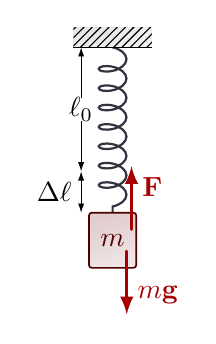
\begin{tikzpicture}
  \def\H{0.25} % ceiling height
  \def\W{1.0}  % ceiling width
  \def\h{0.7}  % mass height
  \def\w{0.6}  % mass width
  \def\y{2.1}  % mass width
  \def\F{0.8}  % force magnitude
  \draw[spring,segment length=7] (0,0) -- (0,-\y);
  \draw[ground] (-\W/2,0) rectangle++ (\W,\H);
  \draw (-\W/2,0) --++ (\W,0);
  \draw[mass] (-\w/2,-\y) rectangle++ (\w,-\h) node[midway] {$m$};
  \draw[force] (0.4*\w,-\y-0.3*\h) --++ (0,\F) node[below right=0] {$\vb{F}$}; %=-k\Delta\ell\vu{y}
  \draw[force] (0.3*\w,-\y-0.7*\h) --++ (0,-\F) node[above right=0] {$m\vb{g}$}; %=mg\vu{y}
  \draw[ell] (-0.4*\W,0) --++ (0,-0.75*\y) node[midway,fill=white,inner sep=0] {$\ell_0$};
  \draw[ell] (-0.4*\W,-0.75*\y) --++ (0,-0.25*\y) node[midway,left=0] {$\Delta\ell$};
\end{tikzpicture}


% VERTICAL spring - extension
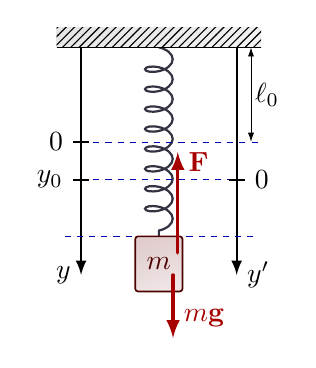
\begin{tikzpicture}
  \def\H{0.25}     % ceiling height
  \def\W{2.6}      % ceiling width
  \def\h{0.7}      % mass height
  \def\w{0.6}      % mass width
  \def\l{0.5*\y}   % rest length without weight
  \def\dl{0.7*\y}  % rest length with weight
  \def\y{2.4}      % mass y position
  \def\xy{0.38*\W} % mass y position
  \def\F{0.8}      % force magnitude
  \draw[spring,segment length=7.2] (0,0) -- (0,-\y);
  \draw[ground] (-\W/2,0) rectangle++ (\W,\H);
  \draw (-\W/2,0) --++ (\W,0);
  \draw[axis] (-\xy,0) --++ (0,-\y-0.7*\h) node[left] {$y$};
  \draw[axis] ( \xy,0) --++ (0,-\y-0.7*\h) node[right] {$y'$};
  \draw[mydashed] (-\xy,-\l) --++ (2.3*\xy,0);
  \draw[mydashed] (-\xy,-\dl) --++ (2*\xy,0);
  \draw[mydashed] (-0.46*\W,-\y) --++ (0.92*\W,0);
  \tick{-\xy,-\l}{0} node[left] {$0$};
  \tick{-\xy,-\dl}{0} node[left] {$y_0$};
  \tick{ \xy,-\dl}{180} node[right] {$0$};
  \draw[mass] (-\w/2,-\y) rectangle++ (\w,-\h) node[midway] {$m$};
  \draw[force] (0.4*\w,-\y-0.3*\h) --++ (0,1.6*\F) node[pos=0.9,right=0] {$\vb{F}$};
  \draw[force] (0.3*\w,-\y-0.7*\h) --++ (0,-\F) node[above right=0] {$m\vb{g}$};
  \draw[ell] (0.45*\W,0) --++ (0,-\l) node[midway,right=-2] {$\ell_0$};
  %\draw[ell] (-0.4*\W,-0.75*\y) --++ (0,-0.25*\y) node[midway,left=1] {$y_0$};
\end{tikzpicture}


% HORIZONTAL doubly extended spring (rest position)
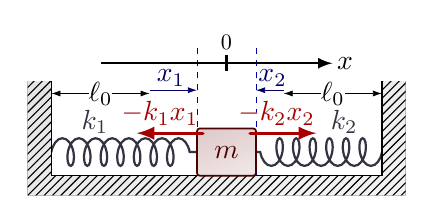
\begin{tikzpicture}
  \def\H{1.2}      % wall height
  \def\T{0.3}      % wall thickness
  \def\W{4.2}      % ground length
  \def\D{0.25}     % ground depth
  \def\h{0.6}      % mass height
  \def\w{0.75}     % mass width
  \def\x{1.85}     % mass x position
  \def\lz{1.25}    % rest length (ell_0)
  \def\ly{0.87*\H} % ell_0 y position
  \def\y{1.19*\H}  % x axis y position
  
  % AXIS
  \draw[mydashed] (\x,0) --++ (0,1.14*\y) (\x+\w,0) --++ (0,1.14*\y);
  \draw[axis] (0.15*\W,\y) --++ (0.7*\W,0) node[right=-2] {$x$};
  \tick{\x+\w/2,\y}{-90} node[scale=0.8,above=-1] {$0$};
  \draw[ell] (0,\ly) --++ (\lz,0) node[midway,fill=white,inner sep=0] {$\ell_0$};
  \draw[ell] (\W,\ly) --++ (-\lz,0) node[midway,fill=white,inner sep=0] {$\ell_0$};
  \draw[dx] (\lz,1.04*\ly) --++ (\x-\lz,0) node[pos=0.45,above=-2] {$x_1$};
  \draw[dx] (\W-\lz,1.04*\ly) --++ (\lz+\x+\w-\W,0) node[pos=0.4,above=-2] {$x_2$};
  
  % SPRINGS & MASS
  \draw[spring,segment length=6] (0,\h/2) --++ (\x,0) node[pos=0.3,above=3] {$k_1$};
  \draw[spring,segment length=6] (\W,\h/2) --++ (\x+\w-\W,0) node[pos=0.3,above=3] {$k_2$};
  \draw[ground] (0,0) |-++ (-\T,\H) |-++ (2*\T+\W,-\H-\D) |-++
                (-\T,\H+\D) --++ (0,-\H) -- cycle;
  \draw (0,\H) -- (0,0) -- (\W,0) --++ (0,\H);
  \draw[mass] (\x,0) rectangle++ (\w,\h) node[midway] {$m$};
  \draw[force] (\x+0.1*\w,0.9*\h) --++ (-0.2*\W,0) node[pos=0.65,above=-1] {\contour{white}{$-k_1x_1$}};
  \draw[force] (\x+0.9*\w,0.9*\h) --++ ( 0.2*\W,0) node[pos=0.40,above=-1] {\contour{white}{$-k_2x_2$}};
  
\end{tikzpicture}


% HORIZONTAL doubly compressed spring (rest position)
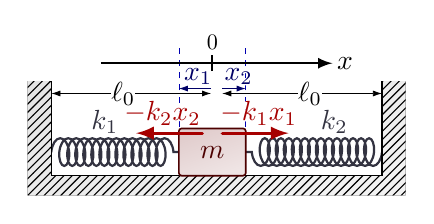
\begin{tikzpicture}
  \def\H{1.2}      % wall height
  \def\T{0.3}      % wall thickness
  \def\W{4.2}      % ground length
  \def\D{0.25}     % ground depth
  \def\h{0.6}      % mass height
  \def\w{0.85}     % mass width
  \def\x{1.62}     % mass x position
  \def\lz{2.03}    % rest length (ell_0)
  \def\ly{0.87*\H} % ell_0 y position
  \def\y{1.19*\H}  % x axis y position
  
  % AXIS
  \draw[mydashed] (\x,0) --++ (0,1.14*\y) (\x+\w,0) --++ (0,1.14*\y);
  \draw[axis] (0.15*\W,\y) --++ (0.7*\W,0) node[right=-2] {$x$};
  \tick{\x+\w/2,\y}{-90} node[scale=0.8,above=-1] {$0$};
  \draw[ell] (0,\ly) --++ (\lz,0) node[pos=0.45,fill=white,inner sep=0] {$\ell_0$};
  \draw[ell] (\W,\ly) --++ (-\lz,0) node[pos=0.45,fill=white,inner sep=0] {$\ell_0$};
  \draw[dx] (\lz,1.06*\ly) --++ (\x-\lz,0) node[pos=0.4,above=-2] {$x_1$};
  \draw[dx] (\W-\lz,1.06*\ly) --++ (\lz+\x+\w-\W,0) node[pos=0.7,above=-2] {\contour{white}{$x_2$}};
  
  % SPRINGS & MASS
  \draw[spring,segment length=2.9] (0,\h/2) --++ (\x,0) node[pos=0.42,above=3] {$k_1$};
  \draw[spring,segment length=2.9] (\W,\h/2) --++ (\x+\w-\W,0) node[pos=0.35,above=3] {$k_2$};
  \draw[ground] (0,0) |-++ (-\T,\H) |-++ (2*\T+\W,-\H-\D) |-++
                (-\T,\H+\D) --++ (0,-\H) -- cycle;
  \draw (0,\H) -- (0,0) -- (\W,0) --++ (0,\H);
  \draw[mass] (\x,0) rectangle++ (\w,\h) node[midway] {$m$};
  \draw[force] (\x+0.65*\w,0.9*\h) --++ ( 0.2*\W,0) node[pos=0.55,above=-1] {\contour{white}{$-k_1x_1$}};
  \draw[force] (\x+0.35*\w,0.9*\h) --++ (-0.2*\W,0) node[pos=0.60,above=-1] {\contour{white}{$-k_2x_2$}};
  %\draw[force] (\x+0.7*\w,0.1*\h) --++ (-0.2*\W,0) node[pos=0.5,below=0] {\contour{white}{$-k_2x_2$}};
  
\end{tikzpicture}


% HORIZONTAL double spring
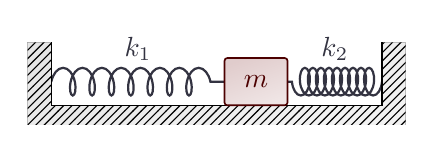
\begin{tikzpicture}
  \def\H{0.8}  % wall height
  \def\T{0.3}  % wall thickness
  \def\W{4.2}  % ground length
  \def\D{0.25} % ground depth
  \def\h{0.6}  % mass height
  \def\w{0.8}  % mass width
  \def\x{2.2}  % mass x position
  \draw[spring,segment length=7.0] (0,\h/2) --++ (\x,0) node[midway,above=4] {$k_1$};
  \draw[spring,segment length=2.9] (\W,\h/2) --++ (\x+\w-\W,0) node[midway,above=4] {$k_2$};
  \draw[ground] (0,0) |-++ (-\T,\H) |-++ (2*\T+\W,-\H-\D) |-++
                (-\T,\H+\D) --++ (0,-\H) -- cycle;
  \draw (0,\H) -- (0,0) -- (\W,0) --++ (0,\H);
  \draw[mass] (\x,0) rectangle++ (\w,\h) node[midway] {$m$};
  %\draw[force] (\x+0.1*\w,0.9*\h) --++ (-0.4*\W,0) node[midway,above=0] {$-k_1\vb{x}$};
  %\draw[force] (\x+0.9*\w,0.9*\h) --++ ( 0.2*\W,0) node[midway,above=0] {$-k_2\vb{x}$};
\end{tikzpicture}


% HORIZONTAL double spring - lengths
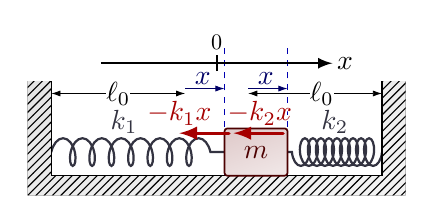
\begin{tikzpicture}
  \def\H{1.2}      % wall height
  \def\T{0.3}      % wall thickness
  \def\W{4.2}      % ground length
  \def\D{0.25}     % ground depth
  \def\h{0.6}      % mass height
  \def\w{0.8}      % mass width
  \def\x{2.2}      % mass x position
  \pgfmathsetmacro\dx{\x+(\w-\W)/2} % extension
  \pgfmathsetmacro\lz{\x-\dx} % rest length (ell_0)
  \def\ly{0.87*\H} % ell_0 y position
  \def\y{1.19*\H}  % x axis y position
  
  % AXIS
  \draw[mydashed] (\x,0) --++ (0,1.14*\y) (\x+\w,0) --++ (0,1.14*\y);
  \draw[axis] (0.15*\W,\y) --++ (0.7*\W,0) node[right=-2] {$x$};
  \tick{\lz+\w/2,\y}{-90} node[scale=0.8,above=-1] {$0$};
  \draw[ell] (0,\ly) --++ (\lz,0) node[midway,fill=white,inner sep=0] {$\ell_0$};
  \draw[ell] (\W,\ly) --++ (\lz+\w-\W,0) node[pos=0.45,fill=white,inner sep=0] {$\ell_0$};
  \draw[dx] (\lz,1.06*\ly) --++ (\dx,0) node[pos=0.45,above=-2] {$x$};
  \draw[dx] (\lz+\w,1.06*\ly) --++ (\dx,0) node[pos=0.45,above=-2] {$x$};
  
  % SPRINGS & MASS
  \draw[spring,segment length=7.0] (0,\h/2) --++ (\x,0) node[pos=0.42,above=3] {$k_1$};
  \draw[spring,segment length=2.9] (\W,\h/2) --++ (\x+\w-\W,0) node[pos=0.5,above=3] {$k_2$};
  \draw[ground] (0,0) |-++ (-\T,\H) |-++ (2*\T+\W,-\H-\D) |-++
                (-\T,\H+\D) --++ (0,-\H) -- cycle;
  \draw (0,\H) -- (0,0) -- (\W,0) --++ (0,\H);
  \draw[mass] (\x,0) rectangle++ (\w,\h) node[midway] {$m$};
  \draw[force] (\x+0.07*\w,0.9*\h) --++ (-0.15*\W,0) node[left=0,above=-1] {\contour{white}{$-k_1x$}};
  \draw[force] (\x+0.93*\w,0.9*\h) --++ (-0.15*\W,0) node[pos=0.47,above=-1] {\contour{white}{$-k_2x$}};
  
\end{tikzpicture}


\end{document}